\documentclass[a4paper,10pt]{article}
\usepackage[utf8]{inputenc}
\usepackage[italian,english]{babel}
\usepackage{graphicx}
\usepackage{url}
\usepackage{wrapfig}

\selectlanguage{italian}

%opening
\title{Gödel}
\author{Riccardo Iaconelli}

\usepackage[dvips, bookmarks, pdfborder={0}, pdftitle={Incompletezza}, pdfauthor={Riccardo Iaconelli}]{hyperref}

\begin{document}
\maketitle

\cleardoublepage
\tableofcontents
\cleardoublepage
\section[Realismo (un'eterna chimera)]{Realismo (un'eterna chimera): ovvero costruisco quindi penso}
Nell'antichità, il ruolo del geometra (mestiere al tempo considerato molto simile all'odierno matematico), era strettamente connesso a quello del filosofo, indagatore della realtà e della natura del mondo. Basti pensare infatti solamente alla celeberrima scritta sulla porta della scuola platonica, che ammoniva: “\textit{non entri chi non è geometra}”. Le forme matematiche erano addirittura le mediatrici tra il mondo delle idee e quello reale.

Che questa frase sia più o meno connessa con l'argomento di questa tesina, poco importa: ciò che è interessante, e che mi preme sottolineare, è che nell'antichità il geometra veniva visto come colui che studiava elementi naturali, reali, che erano dotati di una propria consistenza e vita al di fuori della mente umana.
Quando Euclide riformulò le basi della geometria, creando solide basi che sarebbero state usate fino alla seconda metà dell'ottocento, non si sarebbe mai posto la domanda se tutto il suo lavoro poteva effettivamente essere valido, ovvero coerente con sé stesso. Euclide era solo preoccupato che fosse in grado di dimostrare qualunque teorema effettivamente dimostrabile. Egli infatti pensava, implicitamente, di stare semplicemente descrivendo il mondo naturale: essendo questo esistente, la coerenza e la completezza erano già date per acquisite.

Questa posizione filosofica è anche detta realismo.

\subsection{Il problema dell'infinito e tutti i suoi paradossi}

I Greci avevano già cominciato ad avere qualche esperienza con il concetto di infinito. Ciò nonostante, questo concetto rimaneva problematico, come si può vedere dai vari paradossi ideati in quell'epoca. I più famosi di tutti sono probabilmente i paradossi di Zenone
\cite{wp-paradossi-di-zenone}. Essi implicano spesso il concetto dell'infinito, inteso sia come somma infinita che come elenco infinito di procedimenti.

Consideriamo, ad esempio, il primo paradosso di Zenone contro il movimento. Esso afferma che non si può giungere all'estremità di uno stadio senza prima aver raggiunto la metà di esso, ma prima di raggiungerla si dovrà raggiungere la metà della metà e così via senza quindi mai riuscire a raggiungere l'estremità dello stadio. Questo è un paradosso di non chiara risoluzione.

Infatti, nonostante le moderne tecniche di calcolo infinitesimale abbiano fornito, dal XIX secolo, gli strumenti adatti a risolvere questo tipo di problemi, alcuni filosofi (come Brown o Moorcroft) contestano che i matematici non abbiano ancora risolto il punto centrale del paradosso di Zenone, ossia come fare a gestire infiniti passaggi. Come si fa infatti ad andare dal punto A al punto B, senza che sia possibile stabilire quale sia l'ultimo passo da compiere?

In ogni caso, l'infinito continuò a dar filo da torcere ai matematici fino alla fine del 1800.

Hilbert stesso fu l'autore di un paradosso famoso, che si articola più o meno nel seguente modo: \cite{wp-paradosso-hilbert}
\begin{quote}
Hilbert immagina un hotel con infinite stanze, tutte occupate, ed afferma che qualsiasi sia il numero di altri ospiti che sopraggiungano, sarà sempre possibile ospitarli tutti, anche se il loro numero è infinito.
\end{quote}
Nel caso semplice, arriva un singolo nuovo ospite. 
Allora:
\begin{quote}
L'albergatore sposterà tutti i clienti nella camera successiva (l'ospite della 1 alla 2, quello della 2 alla 3, etc.); in questo modo, benché l'albergo fosse pieno è comunque possibile sistemare il nuovo ospite.
\end{quote}
Un caso meno intuitivo si ha quando arrivano infiniti nuovi ospiti. Sarebbe possibile procedere nel modo visto in precedenza, ma solo scomodando infinite volte gli ospiti (già spazientiti dal precedente spostamento).
Allora Hilbert sostiene che:
\begin{quote}
La soluzione sta semplicemente nello spostare ogni ospite nella stanza con numero doppio rispetto a quello attuale (dalla 1 alla 2, dalla 2 alla 4, etc\dots), lasciando ai nuovi ospiti tutte le camere con i numeri dispari (quindi infinite camere), risolvendo dunque il problema.                                                                                                                                                                                                                                                                                                                                                                                                                                                                                                                                                                                               \end{quote} 
Questo paradosso si può complicare maggiormente:
\begin{quote}
Ci sono infiniti alberghi con infinite stanze tutti al completo. Tutti gli alberghi chiudono, tranne uno. Tutti gli ospiti vogliono alloggiare
nell'unico albergo rimasto aperto. Sarebbe possibile procedere come prima, ma solo scomodando infinite volte gli ospiti.
\end{quote}
Anche in questo caso è possibile risolvere il paradosso, anche se in un modo più complesso e non discutibile in questa sede.

\begin{figure}[t]
 \centering
 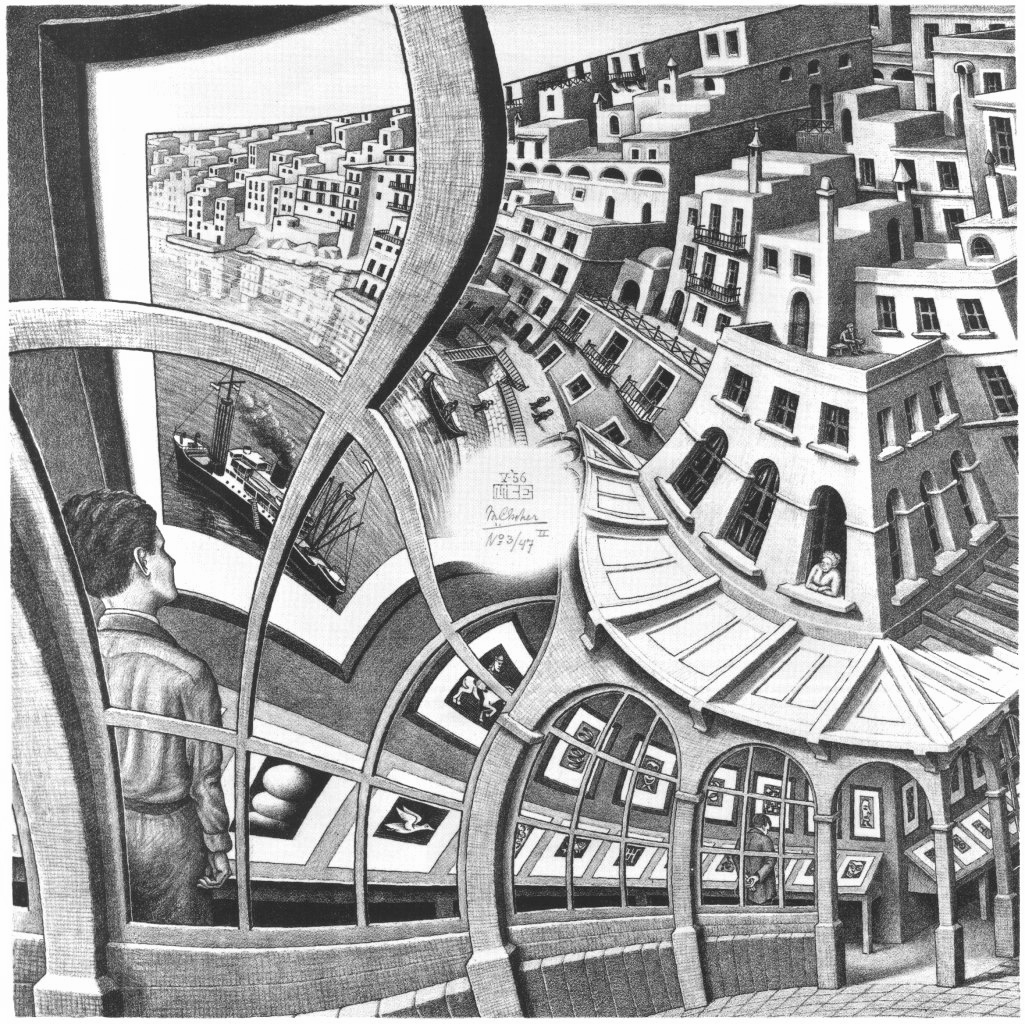
\includegraphics[width=343px]{./pics/escher[3].jpg}
 % escher[3].jpg: 480x480 pixel, 96dpi, 12.70x12.70 cm, bb=0 0 360 360
 \caption{\textsc{M. Escher}, \textit{Galleria di stampe}, 1956.}
\end{figure}

\section[Geometrie non euclidee]{Geometrie non euclidee: ovvero la fine del realismo e la scoperta del potere della mente}

La rassicurante idea realista fu destinata ad essere sconvolta nel XIX secolo, specialmente grazie al lavoro del brillante matematico tedesco David Hilbert.
Hilbert arrivò già a cavallo del 1900, dopo diverse generazione di matematici che, scoperto che Euclide aveva incluso alcuni assiomi ridondanti (ovvero alcuni assiomi non erano altro che teoremi derivabili dagli altri), si erano dati alla “caccia all'errore” all'interno degli Elementi, senza rendersi conto che stavano per spalancare una immensa area di nuova ricerca per la matematica.
Il problema fondamentale che si incontrò riguarda il tentativo di dimostrazione di uno degli assiomi di Euclide. I matematici, dopo aver ridotto gli assiomi da una ventina a cinque, erano alla caccia di una dimostrazione del quinto assioma, basandosi sugli altri quattro. L'intuizione che questo assioma fosse in realtà un teorema viene esclusivamente da un giudizio estetico. Si pensava che fosse un dato di fatto della realtà, che si sarebbe potuto dedurre da semplici definizioni date in precedenza.

Il postulato dice: \cite{wp-elementi-euclide}
\begin{quote}
 Se una retta taglia altre due rette determinando dallo stesso lato angoli interni la cui somma è minore di quella di due angoli retti, prolungando le due rette, esse si incontreranno dalla parte dove la somma dei due angoli è minore di due angoli retti.
\end{quote}
oppure in modo equivalente:
\begin{quote}
 Data una qualsiasi retta r ed un punto P non appartenente ad essa, è possibile tracciare per P una ed una sola retta parallela alla retta r data.
\end{quote}

Essendo falliti tutti i tentativi precedenti di dimostrazioni costruttive, il matematico italiano Gerolamo Saccheri pubblicò nel 1733 un'opera in cui tentava di arrivare ad una dimostrazione dell'assioma per assurdo.

Una dimostrazione per assurdo è una dimostrazione che viene spesso tentata come “ultima spiaggia” dai matematici. La dimostrazione per assurdo procede negando la tesi che si vuole dimostrare e dunque deducendo conseguenze fino a quando si giunge ad un assurdo logico, o ad una contraddizione con assiomi, definizioni, o teoremi precedentemente dimostrati, dimostrando così che la tesi non poteva essere negata e dunque (assumendo che il sistema sia coerente e completo) la tesi è dimostrata.

Alcune scuole di pensiero rigettano in toto questo tipo di dimostrazione, in quanto, pur garantendo l'esistenza di una soluzione, non fornisce ai matematici alcuno strumento per arrivarci effettivamente.

Lobačevskij ritentò circa un cinquantennio dopo, ma aveva già fatto un passo ulteriore rispetto a Saccheri. Siccome, anche dopo un lungo lavoro, non sembrava che si fosse nemmeno apparentemente vicini ad un assurdo, il matematico russo incominciò a supporre che il mondo reale potesse ammettere anche più di una parallela ad una retta data passante per un punto esterno ad essa.

Egli aveva infatti proposto un approcio pragmatico al problema, e sosteneva:
\begin{quote}
Chi può negare, sulla base di effettive misurazioni, che esistano più parallele?
\end{quote}
Pur essendo basata su motivazioni fisiche (egli infatti questionava la possibilità di effettuare misurazioni particolarmente precise), la sua intuizione fu vincente. Oggigiorno Lobačevskij è ricordato come uno dei padri fondatori delle geometrie non-euclidee, pubblicando già nel 1826 i primi i teoremi di quella che oggi è nota come geometria iperbolica. \nocite{wp-geometria-iperbolica}

\section{Hilbert e il formalismo: ovvero penso quindi costruisco}

\begin{wrapfigure}{r}{0.5\textwidth}
 \begin{center}
  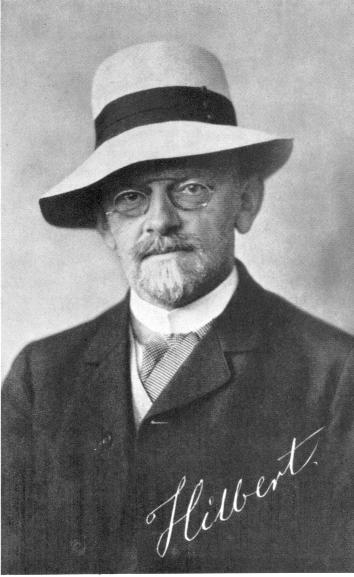
\includegraphics[width=150px]{./pics/hilbert2.jpg}
  % hilbert2.jpg: 354x577 pixel, 72dpi, 12.49x20.36 cm, bb=0 0 354 577  
 \end{center}
\caption{Ritratto di David Hilbert}
\end{wrapfigure}

È a questo punto che David Hilbert entra in gioco.
Il principale merito di Hilbert fu di aver pensato alla geometria e agli enti geometrici, non tanto come enti reali, ma come pure creazioni del nostro pensiero. Invece di descrivere in modo corretto o non corretto una realtà, nella concezione formalista questi sono enti puramente logici e svuotati di ogni significato concreto, tra i quali le uniche relazioni che intercorrono sono quelle che noi decidiamo di fargli intercorrere.
Nel volume \textit{Grundlagen der geometrie} \cite{grundlagen} (1899), Hilbert fondamentalmente riscrive un testo analogo agli \textit{Elementi} di Euclide cercando di fornire alla geometria le solide basi logiche che già analisi e algebra avevano acquisito.

La grande potenza di questo approcio è che, formalizzando ed astraendo tutti i concetti, e rendendolo “un gioco di puri segni”, ogni teorema ricavato può essere applicato a qualunque ente reale che ne provi gli assiomi. Questa concezione è stata essenziale sia per lo sviluppo di teorie come quella della relatività generale, che fa appunto uso di geometrie non euclidee per descrivere l'universo su scale non banali, ma anche per teorie quali quella della probabilità (nella sua formulazione assiomatica), che risolverà gli annosi problemi legati alla sua formulazione classica.


\subsection[L'inizio del formalismo]{Il programma di Hilbert: l'inizio del formalismo}
Analizziamo ora più in dettaglio la genesi del formalismo Hilbertiano.
L'obiettivo di Hilbert era quello di cercare di dare alla matematica basi solide e certe, e nel fare ciò riordinare le varie branche e i vari rapporti che tra esse intercorrevano, cercando una \textquotedblleft teoria prima\textquotedblright\ da cui discendessero tutte le altre.

Per fare ciò occorreva:
\begin{itemize}
 \item Formalizzare tutta la matematica, in modo da identificare in modo rigoroso e preciso le varie entità, e definirne le proprietà e le regole di interazione in modo ben preciso.
 \item Provare la \textbf{completezza} del sistema, cioè che questa formalizzazione provi tutte le asserzioni vere e confuti tutte quelle false.
 \item Provare la \textbf{coerenza} del sistema, cioè provare che non si possano generare asserzioni contraddittorie all'interno del sistema. Questa dimostrazione avrebbe (preferibilmente) dovuto utilizzare metodi finitistici quando applicata ad entità finite.
 \item Provare che ogni risultato ottenuto mediante i simboli \textquotedblleft ideali\textquotedblright\ possa essere ottenuta anche attraverso i simboli reali.
 \item Avere un algoritmo per decidere la verità o la falsità di qualunque asserzione matematica. Questa proprietà è anche detta anche decidibilità.
\end{itemize}

Dunque il lavoro di Hilbert si può semplificare come tentativo estremo di svuotare la matematica da ogni significato estraneo alla pura manipolazione di simboli. Questa posizione sarà ancor più marcata nei suoi allievi, che riterranno la matematica “un puro gioco simbolico senza significato”.
Questa posizione è detta appunto, nella filosofia della matematica, formalismo.
Hilbert riesce a formulare tutta la geometria su di un nocciolo di assiomi da cui dedurre il resto delle dimostrazioni della geometria, servendosi della logica classica come mezzo di deduzione.

\subsection{L'obiettivo di Hilbert: un'assiomatizzazione senza alcun significato}
Tutte queste deduzioni sono fatte in modo rigorosamente formale, senza badare al significato reale di queste dimostrazioni.

Hilbert inoltre pubblica una serie di problemi che la matematica deve risolvere per poter raggiungere l'assiomatizzazione completa. Questi 23 problemi, in parte ancora irrisolti, continuano ad essere una grande sfida per i matematici, e sono considerati di fondamentale importanza per lo sviluppo di questa disciplina.

Il formalismo riscosse molto interesse nei contemporanei di Hilbert. Il primo che riuscì ad arrivare ad una formalizzazione completa fu però il matematico tedesco Gottlob Frege. Egli assiomatizzò completamente l'aritmetica basandola sulla teoria degli insiemi, e pubblicando i suoi risultati nel \textit{Die Grundgesetze der Arithmetik} (Le leggi fondamentali dell'aritmetica). Frege scelse l'aritmetica in quanto era una delle discipline più semplici nella quale praticamente ogni altra ha le sue radici.

\begin{figure}[b!]
 \begin{center}
  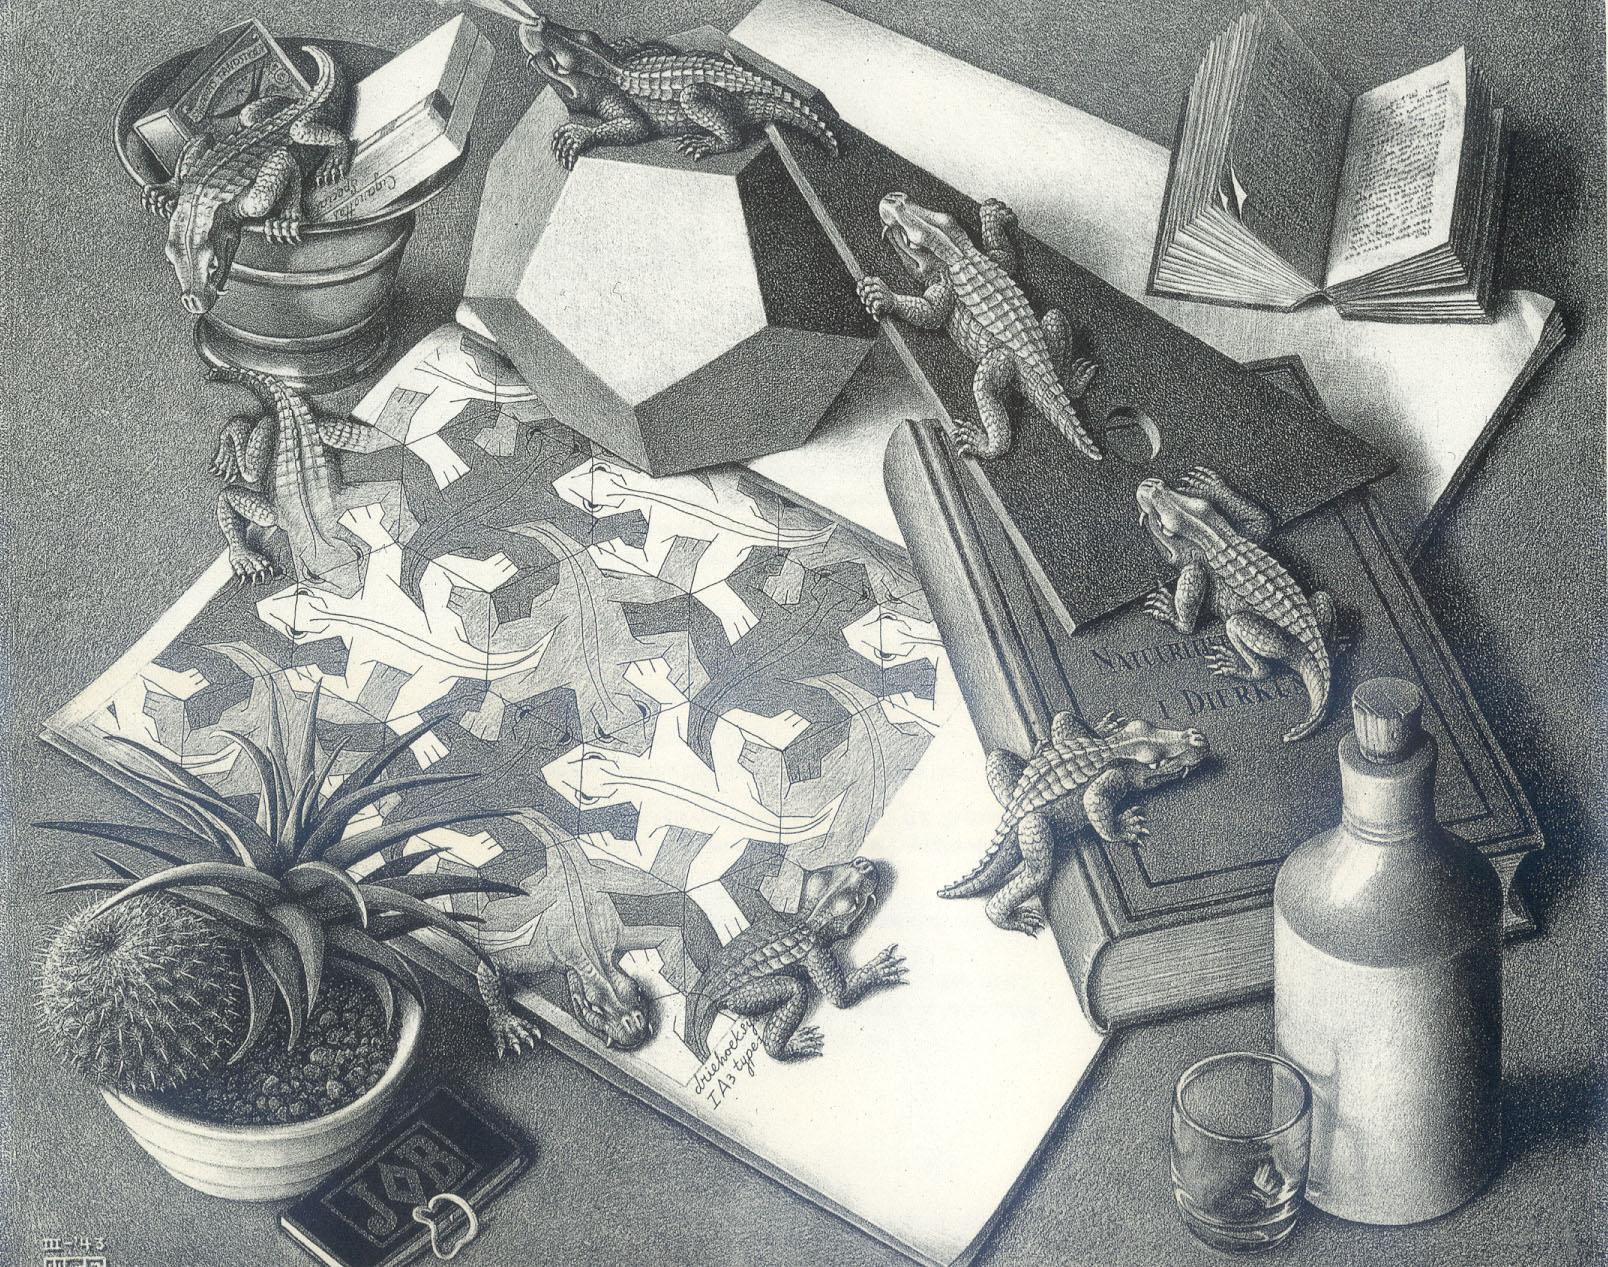
\includegraphics[width=\textwidth,keepaspectratio=true]{./pics/98210399zbOcyG_fs.jpg}  
 \end{center}
 % 98210399zbOcyG_fs.jpg: 1608x1267 pixel, 72dpi, 56.73x44.70 cm, bb=0 0 1608 1267
 \caption{\textsc{M. Escher}, \textit{Rettili}, 1943.}
\end{figure}

\subsubsection[Il problema coerenza]{Il problema del progetto di Hilbert: la coerenza}
Il sistema Hilbertiano però, pur essndo molto potente e pieno di potenzialità rispetto al sistema euclideo, ha da risolvere il problema della coerenza. Il metro di paragone infatti non è più la realtà, autoevidentemente coerente (a detta di Euclide), questi assiomi potrebbero essere contrastanti tra loro, decadendo dunque in un sistema inconsistente, dove si potrebbe dimostrare sia ogni proposizione che il suo contrario. In termini logici: $ \forall x (p(x)\wedge\neg p(x))$.

La questione della coerenza era già stata intuita (ed in parte affrontata) nel passato. Alcuni studiosi erano già riusciti a collegare diverse branche della matematica, collegando di conseguenza anche il problema della coerenza. Un esempio di questo è la geometria analitica, che collega geometria e algebra, e facendo basare l'una sull'altra se ne deduce che, se l'algebra è coerente, allora la geometria è coerente.

Purtroppo però, pochi anni dopo la pubblicazione del \textit{Die Grundgesetze der Arithmetik}, Bertrand Russell formula un paradosso a cui verrà dato il suo nome, che distrugge il lavoro di Frege. Questo paradosso è anche detto “Paradosso del barbiere”.

\subsection{La prima breccia --- il Paradosso del barbiere}
Il paradosso del barbiere è un paradosso molto famoso, che in linguaggio comune potrebbe essere tradotto circa così: (da \cite{wp-paradosso-russel-it})
\begin{quotation}
In un villaggio c'è un unico barbiere. Il barbiere rade tutti (e solo) gli uomini che non si radono da sé. Chi rade il barbiere?                                                                                                                                                                                                                                           \end{quotation} 
Questo paradosso mostra che una delle leggi fondative dell'opera di Frege, la quinta, è inconsistente. Frege purtroppo abbandona il suo lavoro dopo questo rilievo, e dovrà essere proprio Russell, insieme al suo collega Alfred Whitehead, a ricominciarlo. Il frutto di questo lavoro confluirà nel capolavoro dei \textit{Principia Mathematica}, in cui Russell e Whitehead sostituiranno la quinta legge con il più generico principio di Hume. Frege era a conoscenza di questo principio, ma ne avrebbe creato un altro apposito in quanto il principio di Hume sarebbe stato troppo generico. In effetti, il principio di Hume permette l'espressione di formule come \textquotedblleft Giulio Cesare = 2\textquotedblright.

Questo paradosso, più precisamente, può essere formulato nei seguenti termini matematici:
Partendo dal concetto di insieme, che è un concetto primitivo, intuitivo. Un insieme è un “raggruppamento” concettuale qualunque. Siccome posso definire un insieme in tutta libertà, potrò definire l'insieme $\vartheta$ come l'insieme degli insiemi che si non autocontengono. Consideriamo la proprietà di autoappartenenza. Si hanno questi due casi:
\begin{itemize}
 \item Un insieme può essere contenuto in se stesso, come ad esempio l'insieme dei concetti astratti, che è un concetto astratto a sua volta
 \item Un insieme non è contenuto in se stesso. Ad esempio l'insieme delle mele non è una mela a sua volta.
\end{itemize}
Il paradosso nasce dalla domanda: $\vartheta$ è contenuto in sé stesso?
A questo punto infatti ci sono due possibilità:
\begin{itemize}
 \item $\vartheta$ è contenuto in sé stesso. Ma allora, per la definizione stessa di $\vartheta$, non può essere contenuto in sé stesso.
 \item $\vartheta$ non è contenuto in sé stesso.  Ma allora, per la definizione stessa di $\vartheta$, deve essere contenuto in sé stesso.
\end{itemize}

Dunque, $\vartheta$ è contenuto in sé stesso \textbf{se e solo se}  $\vartheta$ non è contenuto in sé stesso.


\subsubsection{Russell dimostra che il programma di Hilbert non può funzionare - La teoria degli insiemi non può essere hilbertianizzata}
La conseguenza più rilevante dell'opera di Russell è il fatto che crei la prima breccia nel programma di Hilbert. Infatti questo paradosso dimostra come la teoria degli insiemi non possa essere completamente assiomatizzata senza cadere nell'inconsistenza.

\section{Gödel e la fine del programma di Hilbert, ovvero pensare e costruire non vanno d'accordo}
Kurt Gödel entra in scena nel 1929, con un teorema fondamentale per il programma di Hilbert, il cosiddetto Teorema di Completezza. Egli dimostra in maniera brillante come esista una corrispondenza tra verità semantica e dimostrabilità logica. In altre parole, mentre è abbastanza facile dimostrare che ogni tautologia è un teorema, Gödel dimostra il contrario, ovvero che ogni teorema è una tautologia, cioè una proposizione necessariamente vera qualunque siano i significati dei predicati utilizzati.

Un'importante conseguenza di questo teorema è che è possibile enumerare con una procedura meccanica tutti i teoremi che derivano da una certa teoria.
Questa, che sembra una banalità, è in realtà una caratteristica fondamentale, che permette di avere un controllo pieno sui vari elementi, e che molti altri oggetti, anche banali, non possiedono. \cite{maraschini-palma}

Ad esempio, è impossibile enumerare in ordine alfabetico l'insieme dei numeri naturali.
Cominciamo considerando solo in numeri tra uno e nove. L'ordine è il seguente:
\begin{enumerate}
  \item cinque
  \item due
  \item nove
  \item otto
  \item quattro
  \item sei
  \item sette
  \item uno
\end{enumerate}

\begin{figure}[b!]
 \centering
 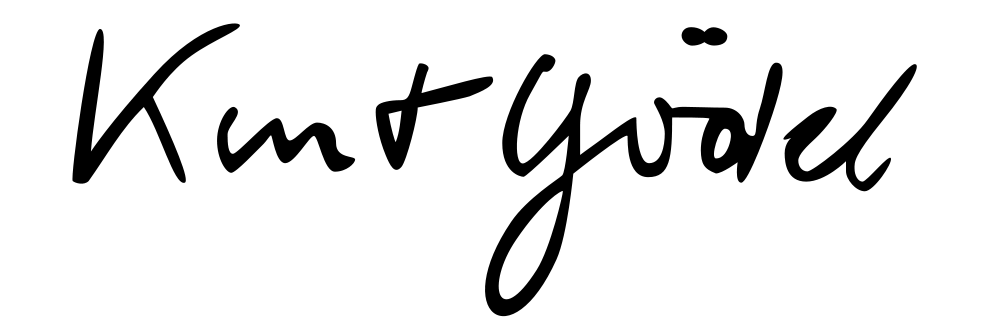
\includegraphics[width=128px]{./pics/128px-KG_signature.png}
 % 128px-Kurt_Gödel_signature.svg.png: 128x43 pixel, 72dpi, 4.52x1.52 cm, bb=0 0 128 43
 \caption{La firma di Kurt Gödel}
\end{figure}

Vediamo facilmente che cercando il precedente del numero due si trova numero cinque. Ma se tentiamo di ordinare in questo modo tutti i numeri naturali, ne troviamo infiniti: c'è infatti il cinque, seguito da tutti i numeri che hanno “cinque-” come radice: il cinquantacinque, il cinquantadue, il cinquecentodue, eccetera\dots

Dunque non esiste un modo per avere, in ordine alfabetico, l'elenco completo di tutti i numeri cardinali. Si dice che non è possibile \textit{enumerare} in questo modo i numeri cardinali. Questo è differente per quanto riguarda le teorie formali, con importantissime conseguenze dal punto di vista della teoria del calcolo.

Il secondo teorema con cui Gödel si presenta, solo l'anno dopo, sulla scena internazionale, è però molto più devastante.

Il suo enunciato è il seguente:

\begin{quote}
  In ogni teoria matematica T sufficientemente espressiva da contenere l'aritmetica, esiste una formula G tale che, se T è coerente, allora né G né la sua negazione $\neg G$ sono dimostrabili in T.
\end{quote} 

E il corollario che ne segue è questo:
\begin{quotation}
  Sia T una teoria matematica sufficientemente espressiva da contenere l'aritmetica: se T è coerente, non è possibile provare la coerenza di T all'interno di T.
\end{quotation}

La dimostrazione segue uno schema abbastanza geniale. Gödel riesce infatti a codificare l'assiomatica dell'aritmetica in un linguaggio interno all'aritmetica stessa, tramite i cosiddetti “numeri di Gödel”.
Questi numeri sono univoci per ogni formula, permettendo dunque di codificarla, e, pur essendo totalmente inutili dal punto di vista pratico, permettono a Gödel di codificare all'interno del sistema aritmetico stesso una formula che affermi la sua propria indimostrabilità.
Fondamentalmente, con qualche semplificazione del caso, si costruisce una formula $P(x)$ che traduca il concetto metamatematico di “$x$ è dimostrabile”, e ad essa, come ad ogni altra formula viene assegnato il suo proprio numero di Gödel, che la identifichi in modo univoco.
A questo punto è sufficiente considerare la formula opposta, quando lavori sul suo proprio numero.
In altre parole, chiamando $G(x)$ la funzione che associa a ogni formula il proprio numero di Gödel, bisogna considerare l'enunciato:

$$
p = \neg P(G(\neg P))
$$

Assumendo che il sistema sia coerente, se $p$ fosse dimostrabile, sarebbe di conseguenza vero. 

Dunque, per la definizione stessa di $\neg P$, la proposizione si può leggere come “La formula con numero di Gödel $G(\neg P)$ è indimostrabile”, dunque “La formula $\neg P$ è indimostrabile”. Ma se così fosse, dunque se $\neg P(x)$ fosse indimostrabile, e ponendo $x = G(\neg P)$, e dunque ritornando all'enunciato p, abbiamo dimostrato che se p è dimostrabile come necessaria conseguenza è indimostrabile.

Non essendo dimostrabile p, assumiamo la sua negazione, $\neg p$, come dimostrabile. Ma se così fosse vorrebbe dire che $G(\neg P)$ non è il numero di Gödel di una formula non dimostrabile, e che dunque $\neg P(x)$ sia dimostrabile. Ma allora ponendo $x = G(\neg P)$, p sarebbe dimostrabile. Ed essendo il sistema consistente, non è possibile che sia p che $\neg p$ siano dimostrabili.

Quindi p non può essere né refutato né accettato all'interno del sistema formale. È \textbf{indecidibile}.

Guardando però questa proposizione dall'esterno del sistema, notiamo che afferma la propria indimostrabilità. E questo è effettivamente vero, perché così accade. Ma non possiamo dimostrarlo all'interno del sistema stesso. Dunque si può dire che un sistema logico formale, per poter essere coerente, deve necessariamente lasciare dei predicati indimostrati, ovvero essere incompleto.

Il corollario dimostra che la formula “L'aritmetica è coerente” all'interno del sistema formale dell'aritmetica è equivalente all'enunciato p, e dunque anch'esso indecidibile. Questo è equivalente a dire:

\begin{quote}
Se un sistema assiomatico può dimostrare la sua stessa coerenza, allora esso deve essere incoerente.
\end{quote}

C'è da notare che le formulazioni di Gödel possono essere applicate soltanto a certi tipi di sistemi logico-formali, ovvero quelli in grado di rappresentare l'aritmetica. È possibile provare la coerenza e completezza assoluta di altri sistemi assiomatici, come l'aritmetica di Presburger (che è un'aritmetica semplificata) o la geometria semplice.

Alcuni studiosi ritengono inoltre che un enunciato, che non può essere dimostrato all'interno di un sistema deduttivo, può essere ben dimostrabile con l'uso di un metalinguaggio.
E che ciò che non può essere dimostrato in quel metalinguaggio può probabilmente essere dimostrato tramite un meta-metalinguaggio.
Questo processo, in teoria, può essere riprodotto ad infinitum in modo ricorsivo. Sarebbe dunque possibile, di volta in volta, aggirare l'ostacolo dell'incompletezza.
Qualche matematico propone anche di usare una assiomatica “scalabile”, ovvero con dei parametri per adattarli alla complessità desiderata.
La validità del teorema di Gödel è stata dimostrata anche in questo caso, ma si potrebbe ritentare.

\section{Gödel, malintesi ed eredità}
Il teorema di Gödel è spesso popolarmente considerato un limite invalicabile alla ricerca matematica, che potrebbe influenzarla in modo importante, e che porrebbe un limite serio alla nostra conoscenza della matematica.
Nonostante le grandi conseguenze filosofiche e personali che ci si potrebbe attendere da una dimostrazione simile, il teorema di Gödel è risultato un teorema particolarmente sterile. A parte alcune applicazioni nella teoria del calcolo (specie nella crittografia), che analizzeremo meglio nel prossimo paragrafo, questo teorema non ha creato quasi alcun problema ai matematici.

In effetti Gödel dimostra che le proposizioni indecidibili sono sì molte, ma fondamentalmente inutili ai fini pratici, o comunque non interessanti.

Inoltre, i sistemi formali che subirebbero le conseguenze del teorema di Gödel sono ben pochi, in quanto dovrebbero: \cite{wp-teo-godel-it}
\begin{enumerate}
 \item Tentare di definire i numeri naturali. Semplicemente usarli non basta.
 \item Essere in grado di esprimere in modo formale il concetto metamatematico \textquotedblleft$x$ è un numero naturale\textquotedblright
\end{enumerate}

Il filosofo John Lucas porta il teorema di Gödel come prova del fatto che la mente umana non sia meccanizzabile. Essa infatti riesce a riconoscere la verità della proposizione gödeliana, dove una qualunque macchina logica non riuscirebbe. Nonostante sia Francois Jacob in \cite{jacob71} che Roger Penrose in \cite{penrose91} gli diano corda, la svista in questo ragionamento è grossolana.

Infatti non è garantito che il cervello sia una macchina coerente, né che sia un sistema logico completo. Nel caso il cervello non fosse coerente, ogni proposizione sarebbe dimostrabile [ $\forall x (T(x)\wedge\neg T(x))$ ] e dunque $p$ diventerebbe addirittura falsa, asserendo la propria indimostrabilità.

...

Altre cattive interpretazioni del teorema vengono descritte nella sezione 6.1 riguardante l'intelligenza artificiale.

\begin{figure}[t!]
 \centering
 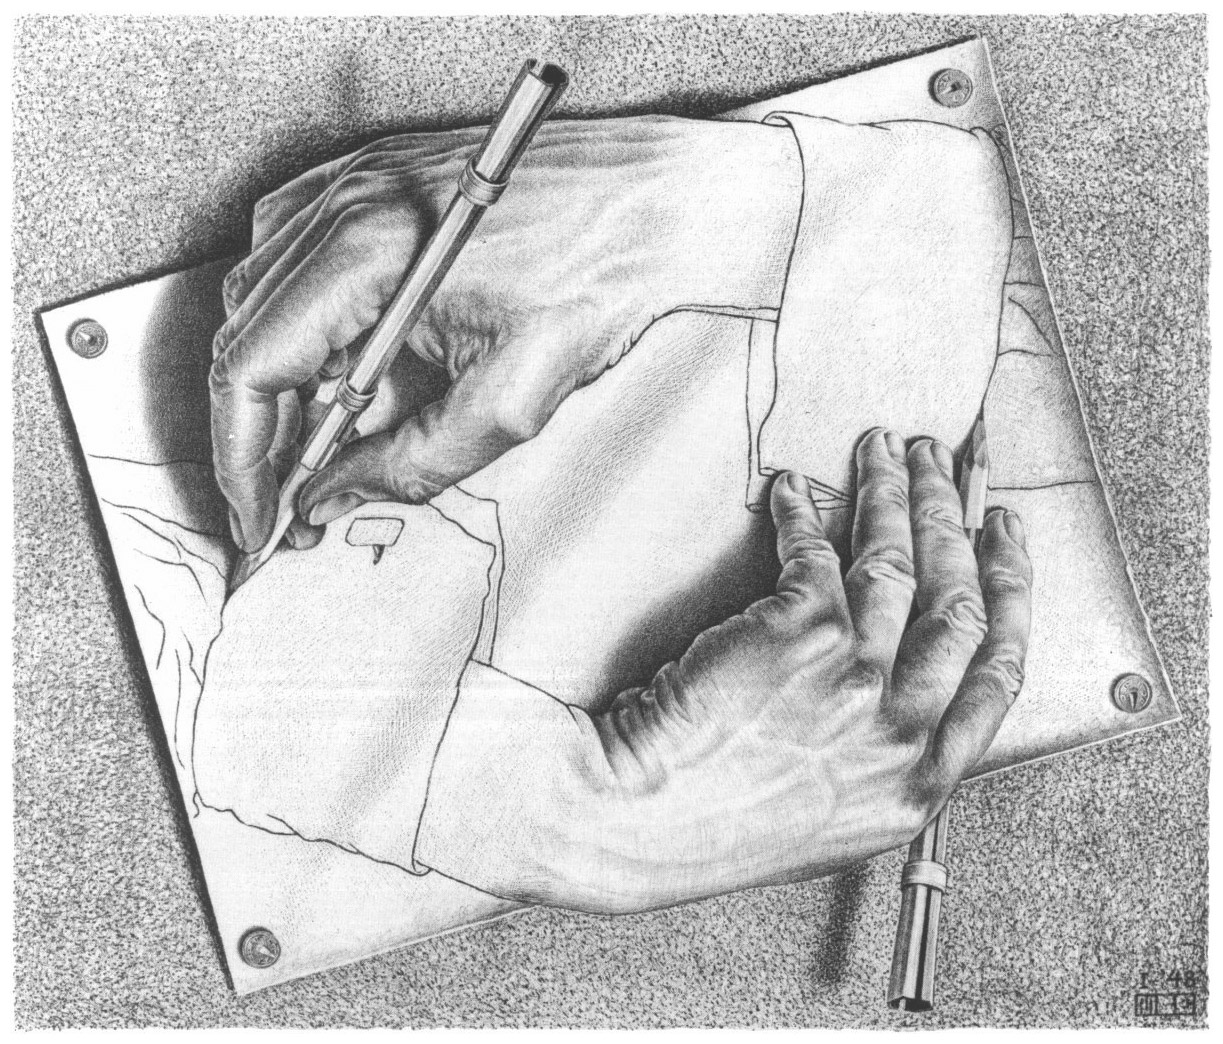
\includegraphics[width=\textwidth]{./pics/drawing_hands.jpg}
 % drawing_hands.jpg: 1223x1044 pixel, 72dpi, 43.14x36.83 cm, bb=0 0 1223 1044
 \caption{\textsc{M. Escher}, \textit{Mani che si disegnano}, 1948.}
\end{figure}

\section{Informatica e teoremi di Gödel}

Interessante è comunque la formulazione del teorema posta in termini informatici, sia quella di Alan Turing, e soprattutto quella da parte di Chaitin.
Il teorema di Turing può essere descritto a parole dicendo che qualunque computer programmabile è incompleto, e non può dunque decidere in anticipo su tutti i problemi che riguardano il suo comportamento.
Dunque, la decidibilità è un concetto più forte della completezza; se così non fosse, si potrebbe scrivere un programma che, enumerando i vari teoremi, dimostri per forza (data la completezza) o la proposizione o la sua negazione (data la coerenza).
Per quanto riguarda la tesi di Chaitin, citiamo il professor Odifreddi, che è molto chiaro a riguardo, nel suo saggio \cite{metamorfosi}:
\begin{quote}
Consideriamo il concetto di numero casuale, tale cioè che qualunque programma che lo stampi non possa avere lunghezza minore di quella del numero stesso: in questo caso la rappresentazione del numero è la sua più corta descrizione, e non è possibile comprimerla sostanzialmente (come invece è possibile, ad esempio, per \textquotedblleft numero costituito da un 1 seguito da un miliardo di 0\textquotedblright, descrizione che richiede sostanzialmente meno di un miliardo di lettere).
Si ha ora la seguente forma del teorema di Gödel: un sistema matematico corretto può provare la casualità soltanto di un numero finito di numeri casuali. Se così non fosse, esisterebbe un programma pn che lavora come segue: si generano i teoremi del sistema formale, fino a trovare un numero casuale di lunghezza maggiore di $n$, e lo si stampa. Poiché i programmi $Pn$ sono tutti uguali eccetto che per la menzione del numero $n$, essi hanno una lunghezza costituita da una parte fissa (una costante $c$) più una parte variabile (di lunghezza uguale alla lunghezza di $n$, cioè $\log(n)$); ed il numero stampato dal programma pn è un numero casuale di lunghezza maggiore di $n$.

Ma se $n$ è sufficientemente grande questo è impossibile: $n$ è infatti maggiore di $c + \log(n)$, e quindi il numero stampato da pn ha lunghezza maggiore di quella di un programma che lo stampa, cioè non può essere casuale.
Il vantaggio della formulazione di Chaitin nei confronti di quelle di Gödel e Turing è duplice: essa non richiede autoriferimenti nella dimostrazione, ed esibisce enunciati veri ma non dimostrabili di interesse matematico (e non soltanto logico).
\end{quote}

\selectlanguage{english}
\subsection{[English] Gödel and the A.I.}

For what concerns the A.I., Gödel's incompleteness theorem could have, at first sight, some intriguing consequences.

An intelligent machine is, after all, simply a logical machine, which has some axioms, and which can then form judgments by evaluating certain inputs and following some rules, which could be either axioms (the programmed rules) or theorems (rules inferred from experience).

Here we will analyze the posistion of two important intellectuals who used the theorem in order to argumentate either in favour or against it. They are respectively Douglas Hofstader and Roger Penrose.

R. Penrose utilizes the fallant argument that J. Lucas proposed about the man being superior to any attempt to mechanize human's mind. R. Penrose uses this argument \cite{penrose91} to prove the fact that no perfect A.I. can ever be built. However, we have already seen that this argument has very little basis in a previous section.

D. Hofstader sets himself on a completely different position. In his well known \textit{Gödel, Escher, Bach}\cite{geb}, he tries to argument in favor of the various immense \textit{possibilities} of machines built by humans, but does so using a theorem that talks of their \textit{limitations}.
While the argument in itself is very correct (since Hofstader correctly interpets Gödel's theorem and its implication) it is also quite useless.

Infact, as Hofstader himself is forced to admit, we can only assert that Gödel's theorem does not \textit{exclude} the possibility of creating intelligent machines, but on the other hand without \textit{demonstrating} it either. While these machines could, in theory, replicate the functions on the human brain, we have no implications whatsoever coming directly from Gödel's work.

In the end, the error of both books is to try to demonstrate a thesis, which they can't find, since Gödel's theorem is, as a matter of fact, a very technical theorem.

Gödel's theorem does say what we can know of math (and the answer is: very little), but it does not say anything about the usefulness of these prepositions. In the same way as an immense quantity of real numbers cannot be defined, this doesn't mean that real numbers are unuseful, or that our knowledge of them is limited in any practical way: on the contrary, all the interesting numbers that we need are defined, and probably this is the same also all interesting mathematical prepositions. We cannot prove that the insiemistic theories are coherent, but it most probably is; and most importantly, the theory works beautifully.

Besides, what best proof of self knowledge than knowing one's own limits?

\selectlanguage{italian}
\section{Reminescenze filosofiche}

Il teorema di incompletezza di Gödel non è però una completa novità del Novecento. Già Immanuel Kant, sia nella \textit{Critica della ragion pura} \cite{critica-ragion-pura} che nei \textit{Prolegomeni ad ogni metafisica futura} \cite{prolegomeni}, propone tra i suoi punti fondamentali l'incompletezza della ragione.

Il sistema di Kant può essere sommariamente descritto parlando delle \textquotedblleft idee trascendentali\textquotedblright, che non sono altro che i concetti derivanti dalle categorie di relazione, quando sono portate all'estremo. Ad esempio, il limite della disgiunzione è una disgiunzione omnicomprensiva che abbracci tutto, e viene chiamato \textit{mondo}.

Ora, i filosofi razionalisti quali Leibniz e Cartesio, basando la loro filosofia sulla ragione (oltre che sul dubbio sistematico), avevano tentato di arrivare a una dimostrazione di queste idee trascendentali.
Kant però mostra come ogni dimostrazione di queste sia inevitabilmente destinata a fallire. Infatti, mediante le quattro antinomie, mostra che le idee trascendentali sono contraddittorie, e ne deduce che, richiedendo la completezza della ragione, si cade inevitabilmente nell'inconsistenza.

Sempre il prof. P. Odifreddi sostiene \cite{metamorfosi} che:
\begin{quotation}
La conclusione di Kant si può riformulare dicendo che se la ragione vuole essere consistente, non può essere completa (nel senso di
poter decidere ogni problema che essa si ponga). Se si sostituisce 'ragione' con 'sistema matematico', si ottiene precisamente una
formulazione del teorema di Gödel. E anche la dimostrazione di questo procede, in essenza, come quella di Kant: dato un
sistema matematico, si considera un'idea trascendentale ottenuta come limite della non dimostrabilità nel sistema (una formula
che dica di se stessa di non essere dimostrabile nel sistema), e si mostra che se il sistema è completo (cioè decide ogni formula,
dimostrando o essa stessa o la sua negazione) allora si cade nell'inconsistenza.

\end{quotation}

Questo non stupisce, visto che Gödel stesso sottolineò come avesse raggiunto i suoi risultati concentrandosi \textquotedblleft\textit{su appropriate nozioni filosofiche tradizionali, aggiungendo eventualmente un pizzico di precisione}\textquotedblright \cite{odifreddi-e-ia}


\cleardoublepage

\section{Riconoscimenti e bibliografia}
Questa tesina è stata realizzata attraverso l'uso esclusivo di Software Libero.

\nocite{geb}

\bibliographystyle{siam}
\bibliography{tesina}

\listoffigures

\end{document}
